\documentclass{assets/utmreport}

\usepackage{booktabs,amssymb,float,graphicx,adjustbox,array}
\usepackage{tikz}\usetikzlibrary{positioning,arrows.meta}
\usepackage{newunicodechar}
\newfontfamily\diafont{Liberation Serif}
\newunicodechar{ș}{{\diafont ș}}\newunicodechar{ț}{{\diafont ț}}\newunicodechar{Ș}{{\diafont Ș}}\newunicodechar{Ț}{{\diafont Ț}}

\hypersetup{hidelinks,hypertexnames=false,pdfauthor={Lucian-Adrian Gavril}}

\selectlanguage{english}

\utmlogo{assets/utm-logo.jpeg}

\institution{Technical University of Moldova}
\faculty{Faculty of Computers, Informatics, and Microelectronics}
\department{Department of Software Engineering}
\studyprogramme{Software Engineering Study Programme}
\documenttype{Report on laboratory work no. 12}
\reporttitle{Operating Systems}
\reportsubtitle{Producer, Consumer and the Other Tools}
\student{Lucian-Adrian Gavril}{FAF-241}
\supervisor{Reițman Patricia}{univ. assist.}
\cityyear{Chișinău}{2026}

\newcommand{\shot}[2]{\begin{figure}[H]\centering\adjustbox{scale=0.6,max width=\linewidth,max height=0.78\textheight}{\includegraphics{assets/#1}}\caption{#2}\end{figure}}
\lstset{basicstyle=\ttfamily\small,columns=fullflexible,keepspaces=true,frame=single,framerule=0.4pt,xleftmargin=1em,xrightmargin=1em}

\begin{document}
\sloppy
\makeutmreporttitlepage
{\small\tableofcontents}
\clearpage

\utmintroduction
\textbf{Purpose of the work.} To make the synchronisation tools of Lab~11 work together on the classic problems of every operating systems course. A bounded buffer between a fast producer and a slow consumer uses two counting semaphores and a mutex; the ordering problem of Lab~11 is solved again with a condition variable; readers and writers share data with two semaphores; and two mutexes taken in opposite order build a deadlock that is then removed.

\textbf{Environment.} Debian GNU/Linux 13, Linux kernel 7.2, GCC 14.2, on an Intel Core i7-1355U with 12 logical CPUs. Every program is compiled with \texttt{gcc -Wall -pthread} and builds with no warning. The handed-in sources are the programs of the brief (\texttt{deadlock.c} in its fixed form); each also sets \texttt{stdout} to line buffering, so the order of the lines in a figure is the real order of the \texttt{printf} calls. The experiments of the Observe questions are built from the same sources with \texttt{-D} flags: \texttt{prodcons\_swapped}, \texttt{condvar\_if}, \texttt{deadlock\_orig} and \texttt{deadlock\_nosleep} (\texttt{make} builds all of them). Every terminal figure is the real output of the commands shown in it; the raw text is in \texttt{evidence/}.

\chapter{Producer and consumer}

\section{A buffer of four slots}
Three tools share the work: \texttt{empty} counts the free slots and starts at 4, \texttt{full} counts the filled slots and starts at 0, and a mutex protects the buffer and its indexes \texttt{in} and \texttt{out}. The run matches the expected output line for line (Figure~1.1). The producer puts four items at once and is then stopped; from there on each \texttt{take} of the slow consumer (300~ms per item) allows exactly one more \texttt{put}, and the last four \texttt{take}s empty the buffer. \texttt{in buffer} stays between 0 and 4.
\shot{1_prodcons.png}{prodcons: the buffer never holds more than 4}

\section{The mutex taken first}
In \texttt{prodcons\_swapped} the producer locks the mutex \emph{before} \texttt{sem\_wait(\&empty)}. It puts items 1 to 4 and then the program stops forever; \texttt{timeout} kills it after 5~seconds with exit code 124 (Figure~1.2). Not a single \texttt{take} is printed.
\shot{1_swapped.png}{The lock taken before sem\_wait(\&empty): the program stops at a full buffer}

\section*{Observe 1}
\textbf{1. The producer is fast, yet ``in buffer'' never goes above 4. Which call stops it?}
\texttt{sem\_wait(\&empty)}. After four \texttt{put}s, \texttt{empty} is 0 and the producer sleeps there until the consumer's \texttt{sem\_post(\&empty)} frees a slot.

\textbf{2. Who waits at the start? Which call makes it wait?}
The consumer. It is created first and calls \texttt{sem\_wait(\&full)} while \texttt{full} is still 0; it sleeps until the producer's first \texttt{sem\_post(\&full)}.

\textbf{3. Lock before sem\_wait(\&empty): what happens when the buffer is full, and why?}
A deadlock. With the buffer full, the producer holds the mutex and sleeps in \texttt{sem\_wait(\&empty)}. The consumer passes \texttt{sem\_wait(\&full)} but blocks on \texttt{pthread\_mutex\_lock}. The producer waits for a \texttt{sem\_post(\&empty)} that only the consumer can make, and the consumer waits for an unlock that only the producer can make. The rule is to wait on the counting semaphore first and to hold the mutex only around the buffer itself, never while sleeping.

\chapter{The condition variable}

\section{order.c again}
\texttt{condvar.c} solves the problem of \texttt{order.c} from Lab~11 with a mutex, an ordinary variable \texttt{ready} and a condition variable \texttt{changed}. B takes the mutex, finds \texttt{ready == 0}, prints that it sleeps and calls \texttt{pthread\_cond\_wait}, which releases the mutex while B sleeps. One second later A sets \texttt{ready = 1} under the mutex and signals; B wakes with the mutex taken again, checks \texttt{ready} once more and reads \texttt{"hello"} (Figure~2.1, first run). With \texttt{if} instead of \texttt{while} (\texttt{condvar\_if}, second run) the output is identical.
\shot{2_condvar.png}{condvar with while, then with if}

\section*{Observe 2}
\textbf{1. Which variable remembers that the message is ready?}
\texttt{ready}, an ordinary integer protected by \texttt{lock}. The condition variable has no memory: a signal sent while nobody waits is lost. That is why B tests \texttt{ready} before it sleeps, and why A changes it under the same mutex.

\textbf{2. Replace while with if. Does it still work here?}
Yes (Figure~2.1). There is one writer, one reader and one signal, sent after \texttt{ready} became 1, so the single wake-up B receives is the correct one.

\textbf{3. Then why do we write while?}
Because waking up does not prove that the condition is true. POSIX allows \texttt{pthread\_cond\_wait} to return without any signal (a spurious wake-up). Even after a real signal, another thread can take the mutex before the woken one and use the condition up: a second reader that sets \texttt{ready} back to 0, or several consumers woken by \texttt{pthread\_cond\_broadcast} for a single item. \texttt{while} checks the condition again every time the thread wakes.

\chapter{Readers and writers}

\section{Three runs}
\texttt{readers.c} starts writer~1, three readers and writer~2. In all three runs the three readers are inside together (\texttt{readers inside: 1, 2, 3}) and every writer prints alone (Figure~3.1). The order depends on the scheduler: in the second run writer~1 started first and the readers read 10, as in the brief; in the first and third runs the readers entered first and read 0, and both writers followed after the last reader had left.
\shot{3_readers.png}{readers: three readers together, every writer alone}

The third run also shows a small detail: \texttt{readers inside: 3} is printed before \texttt{readers inside: 2}. The \texttt{printf} reads \texttt{readers} outside \texttt{rlock}, so it prints the value of the moment, which another reader may already have changed. Here it is only display, but it is the same unprotected read that Question~2 is about.

\section*{Observe 3}
\textbf{1. Which two lines of reader() allow three readers together and a writer alone?}
\begin{lstlisting}[language=C]
if (++readers == 1) sem_wait(&room);  /* the first reader in */
if (--readers == 0) sem_post(&room);  /* the last reader out */
\end{lstlisting}
Only the first reader takes \texttt{room}; the next ones see that readers are already inside and enter without it. The group of readers holds \texttt{room} as one and returns it when the last reader leaves. A writer needs \texttt{room} for itself, so it can never be inside together with readers or with another writer.

\textbf{2. Why does readers need its own lock?}
\texttt{++readers} and \texttt{--readers} are load--add--store, the race of Lab~11, and the test \texttt{== 1} or \texttt{== 0} must happen in the same step as the change. Without \texttt{rlock}, two arriving readers can both see the count become 1 and both call \texttt{sem\_wait(\&room)}, so the second one blocks although it is allowed in. Two leaving readers can lose a decrement: the count never comes back to 0, \texttt{room} is never released and the writers wait forever; or it reaches 0 too early, and a writer changes \texttt{value} while a reader is still reading.

\textbf{3. Readers that keep arriving: what happens to writer~2?}
It starves. While at least one reader is inside, \texttt{readers} never falls to 0 and \texttt{room} is never posted, so writer~2 waits in \texttt{sem\_wait(\&room)} indefinitely, although nothing is deadlocked and the readers keep making progress. This solution favours readers; the usual remedy is an extra ``turnstile'' semaphore that a waiting writer holds, so that newly arriving readers queue behind it.

\chapter{Build a deadlock, then remove it}

\section{The circle}
In \texttt{deadlock\_orig}, \texttt{one()} locks A then B and \texttt{two()} locks B then A, with \texttt{sleep(1)} between the two locks. Both threads print their first line, and then nothing happens: \texttt{timeout} kills the program after 5~seconds, \texttt{exit code: 124} (Figure~4.1).
\shot{4_deadlock.png}{The original order: both threads stop, exit code 124}

\section{The fix}
In the handed-in \texttt{deadlock.c}, \texttt{two()} takes A first and then B, the same order as \texttt{one()} (its message now says what it really holds: \texttt{I have A, I want B}). Whichever thread gets A first finishes, then the other one runs; the program prints \texttt{done} and exits with 0 (Figure~4.2).
\shot{4_fixed.png}{The same order in both threads: done, exit code 0}

\section{Without the sleeps}
\texttt{deadlock\_nosleep} is the original order with the two \texttt{sleep(1)} lines removed (Figure~4.3). On 12 CPUs, 4 of 10 runs hung, and 53 of 100. Pinned to a single CPU with \texttt{taskset -c 0}, all 100 runs finished. Two more sessions of 100 runs, a few minutes later, hung 72 and 68 times (Figure~4.4): the share itself changes from session to session.
\shot{4_nosleep.png}{Without sleep(1): 10 runs, 100 runs on 12 CPUs, 100 runs on one CPU}
\shot{4_nosleep_sessions.png}{Two more sessions of 100 runs: 72 and 68 hang}

\section*{Observe 4}
\textbf{1. Which thread holds which mutex and waits for which? Draw the circle.}
\begin{center}
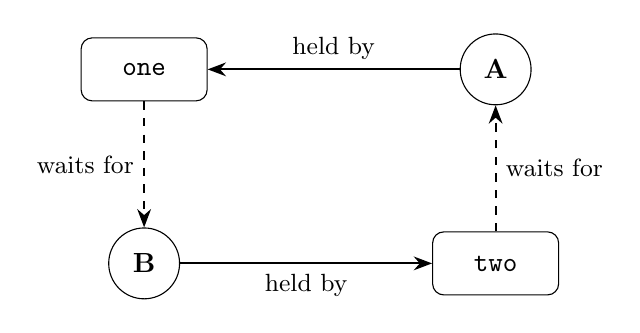
\begin{tikzpicture}[node distance=1.6cm and 3.2cm, thr/.style={draw,rounded corners,minimum width=1.6cm,minimum height=0.8cm,font=\ttfamily}, mtx/.style={draw,circle,minimum size=0.9cm,font=\bfseries}, >=Stealth, every edge quotes/.style={font=\small,auto}]
\node[thr] (one) {one};
\node[mtx, right=of one] (A) {A};
\node[thr, below=of A] (two) {two};
\node[mtx, below=of one] (B) {B};
\draw[->,thick] (A) to node[above,font=\small] {held by} (one);
\draw[->,thick,dashed] (one) to node[left,font=\small] {waits for} (B);
\draw[->,thick] (B) to node[below,font=\small] {held by} (two);
\draw[->,thick,dashed] (two) to node[right,font=\small] {waits for} (A);
\end{tikzpicture}
\end{center}
\texttt{one} holds A and waits for B; \texttt{two} holds B and waits for A. The waits close a circle one $\to$ B $\to$ two $\to$ A $\to$ one, so neither thread can ever continue.

\textbf{2. Without sleep(1), does it still always hang? Why is that worse?}
No. On 12 CPUs it hung in 4 of 10 runs, and in 53, 72 and 68 of 100 in three sessions: the \texttt{printf} between the two locks still leaves a window in which the other thread can take its first lock. On one CPU all 100 runs finished, because a thread usually takes both locks before it is preempted. With \texttt{sleep(1)} the deadlock is certain and is found at the first test. Without it, the outcome depends on timing, core count and load: the program can pass every test on one machine and hang later on another. The bug is the same; it has only become intermittent, which makes it much harder to reproduce and to debug.

\textbf{3. Why can taking the locks in the same order never deadlock?}
If all threads take the locks in one global order, a thread that holds a lock only ever waits for a lock that comes later in that order, so the chain of waits always moves forward and can never close into a circle.

\section*{Answers in brief}
\begin{tabular}{@{}p{0.38\linewidth}p{0.56\linewidth}@{}}
\toprule
Experiment & Result \\
\midrule
\texttt{prodcons} & never more than 4 in the buffer; the consumer waits first \\
lock before \texttt{sem\_wait(\&empty)} & deadlock at a full buffer, exit code 124 \\
\texttt{condvar} with \texttt{if} & works here, one signal for one waiter \\
\texttt{readers} & up to 3 readers together, writers always alone \\
\texttt{deadlock} original / fixed & exit 124 / \texttt{done}, exit 0 \\
no \texttt{sleep(1)} & 53, 72, 68 of 100 hang on 12 CPUs; 0 of 100 on one CPU \\
\bottomrule
\end{tabular}

\utmconclusions
The tools of Lab~11 combine into the standard solutions. In the bounded buffer the two counting semaphores carry the state (free and filled slots) and the mutex only protects the buffer; swapping two lines, so that a thread slept on a semaphore while holding the mutex, turned the working program into a deadlock at the first full buffer.

A condition variable separates the two jobs that a semaphore does together: the state lives in an ordinary variable under a mutex, and the condition variable is only where a thread sleeps. Because a wake-up is only a hint, the state is checked in a \texttt{while} loop; the \texttt{if} version worked in this program only because it had exactly one waiter and one signal.

The readers--writers solution allowed three readers at once and kept every writer alone, at the price of possible starvation of the writers. The deadlock needed exactly the four conditions of the theory, and breaking one of them, the circular wait, by a single global lock order removed it. The run without \texttt{sleep(1)} was the most instructive: the same wrong code hung in roughly half to three quarters of the runs on twelve CPUs, a different share in every session, and never on one CPU, which is why lock-order bugs must be prevented by design rather than found by testing.

\end{document}
